\begin{frame}
	\Huge Brücken und Separatoren
\end{frame}

\begin{frame}
	\frametitle{Brücken und Separatoren}
	\framesubtitle{Definition}
	\begin{KITinfoblock}{Separatoren und Brücken in ungerichteten Graphen}
		Sei $G = (V,E)$ ein ungerichteter Graph.
	\begin{itemize}
		\item  Ein Knoten $v \in V$ heißt \textbf{Separator} von $G$, wenn  durch sein Entfernen bestehende Zusammenhangskomponenten aufgetrennt werden.
		\item  Eine Kante $\{u,v\} \in E$ heißt \textbf{Brücke}, wenn durch ihr Entfernen  $u$ und $v$ in verschiedenen Zusammenhangskomponenten liegen.
	\end{itemize}
	\end{KITinfoblock}
	
\end{frame}
\begin{frame}
	\frametitle{Brücken und Separatoren}
	\framesubtitle{Beispiel}
	\includegraphics[scale = 0.5]<1-1>{Bruecke_Separator_Beispiel_1.pdf}
	\includegraphics[scale = 0.5]<2-2>{Bruecke_Separator_Beispiel_2.pdf}
	\includegraphics[scale = 0.5]<3-3>{Bruecke_Separator_Beispiel_3.pdf}
\end{frame}

\begin{frame}
	\frametitle{Brücken und Separatoren}
	\framesubtitle{Algorithmen}
	\begin{itemize}
		\item Naive Herangehensweise:
			\begin{enumerate}
				\item Entferne einen Knoten/Kante
				\item Prüfe mittels DFS/BFS ob sich eine neue Zusammenhangskomponente ergeben hat
				\item Wiederhole Schritt 1 für alle Knoten/Kanten
			\end{enumerate}
			\item Laufzeit: $\mathcal{O}(|V| \cdot (|V| + |E|))$ bwz. $\mathcal{O}(|E| \cdot (|V| + |E|))$
			\item Es existiert Algorithmus  in  $\mathcal{O}(|V| + |E|)$
			\item Basiert auf DFS und ähnelt Algorithmus zum Finden von SCCs
	\end{itemize}
\end{frame}
\begin{frame}
	\frametitle{Brücken und Separatoren}
	\framesubtitle{Idee des effizienten Algorithmus'}
	\begin{itemize}
		\item Führe eine DFS im Graph durch.
		\item Besuchte Knoten erhalten zwei Nummern:
		\pause
			\begin{enumerate}
				\item \textbf{dfs\_num(u):} Speichert Schritt, in dem Knoten $u$ von DFS besucht wurde.
				\item \textbf{dfs\_low(u):} Niedrigster Wert von \textbf{dfs\_low}, der von Knoten $u$ aus erreicht werden kann. 
			\end{enumerate}
			\pause
			\item Wenn \textbf{dfs\_low(v)} $\geq$ \textbf{dfs\_num(u)}, dann ist $u$ ein Separator 
			\pause
			\begin{itemize}
				 \item Von $v$ kann kein Knoten $w$ "vor" $u$ erreicht werden.
				 \item "vor" bedeutet: (\textbf{dfs\_num($w$)} $>$ \textbf{dfs\_num($u$)})
				 \item Um Knoten $w$ "vor" $u$ zu erreichen, muss man durch $u$ laufen.
				 \item $\Rightarrow$ $u$ teilt Graph in zwei Zusammenhangskomponenten.
				 \item (Spezialfall: Gilt nicht, wenn $u$ Wurzel der DFS)
			\end{itemize} 
	\end{itemize}
\end{frame}
\begin{frame}
		\frametitle{Brücken und Separatoren}
		\framesubtitle{Idee des effizienten Algorithmus'}
	\begin{itemize}
	\item Besuchte Knoten erhalten zwei Nummern:
	\begin{enumerate}
		\item \textbf{dfs\_num(u):} Speichert Schritt, in dem Knoten $u$ von DFS besucht wurde.
		\item \textbf{dfs\_low(u):} Niedrigster Wert von \textbf{dfs\_low}, der von Knoten $u$ aus erreicht werden kann. 
	\end{enumerate}
	\pause
	\item Wenn \textbf{dfs\_low(v)} $>$ \textbf{dfs\_num(u)}, dann ist $\{u,v\}$ eine Brücke
	\begin{itemize}
		\item Von $v$ kann Knoten $v$ nur über die Kante ${u,v}$ erreicht werden.
		\item Ansonsten \textbf{dfs\_low(v)} $seq$ \textbf{dfs\_num(u)}.
		\item $\Rightarrow$ $\{u,v\}$ teilt Graph in zwei Zusammenhangskomponenten.
	\end{itemize} 
\end{itemize}
\end{frame}
\begin{frame}
	\frametitle{Brücken und Separatoren}
	\framesubtitle{Illustration des Algorithmus'}
	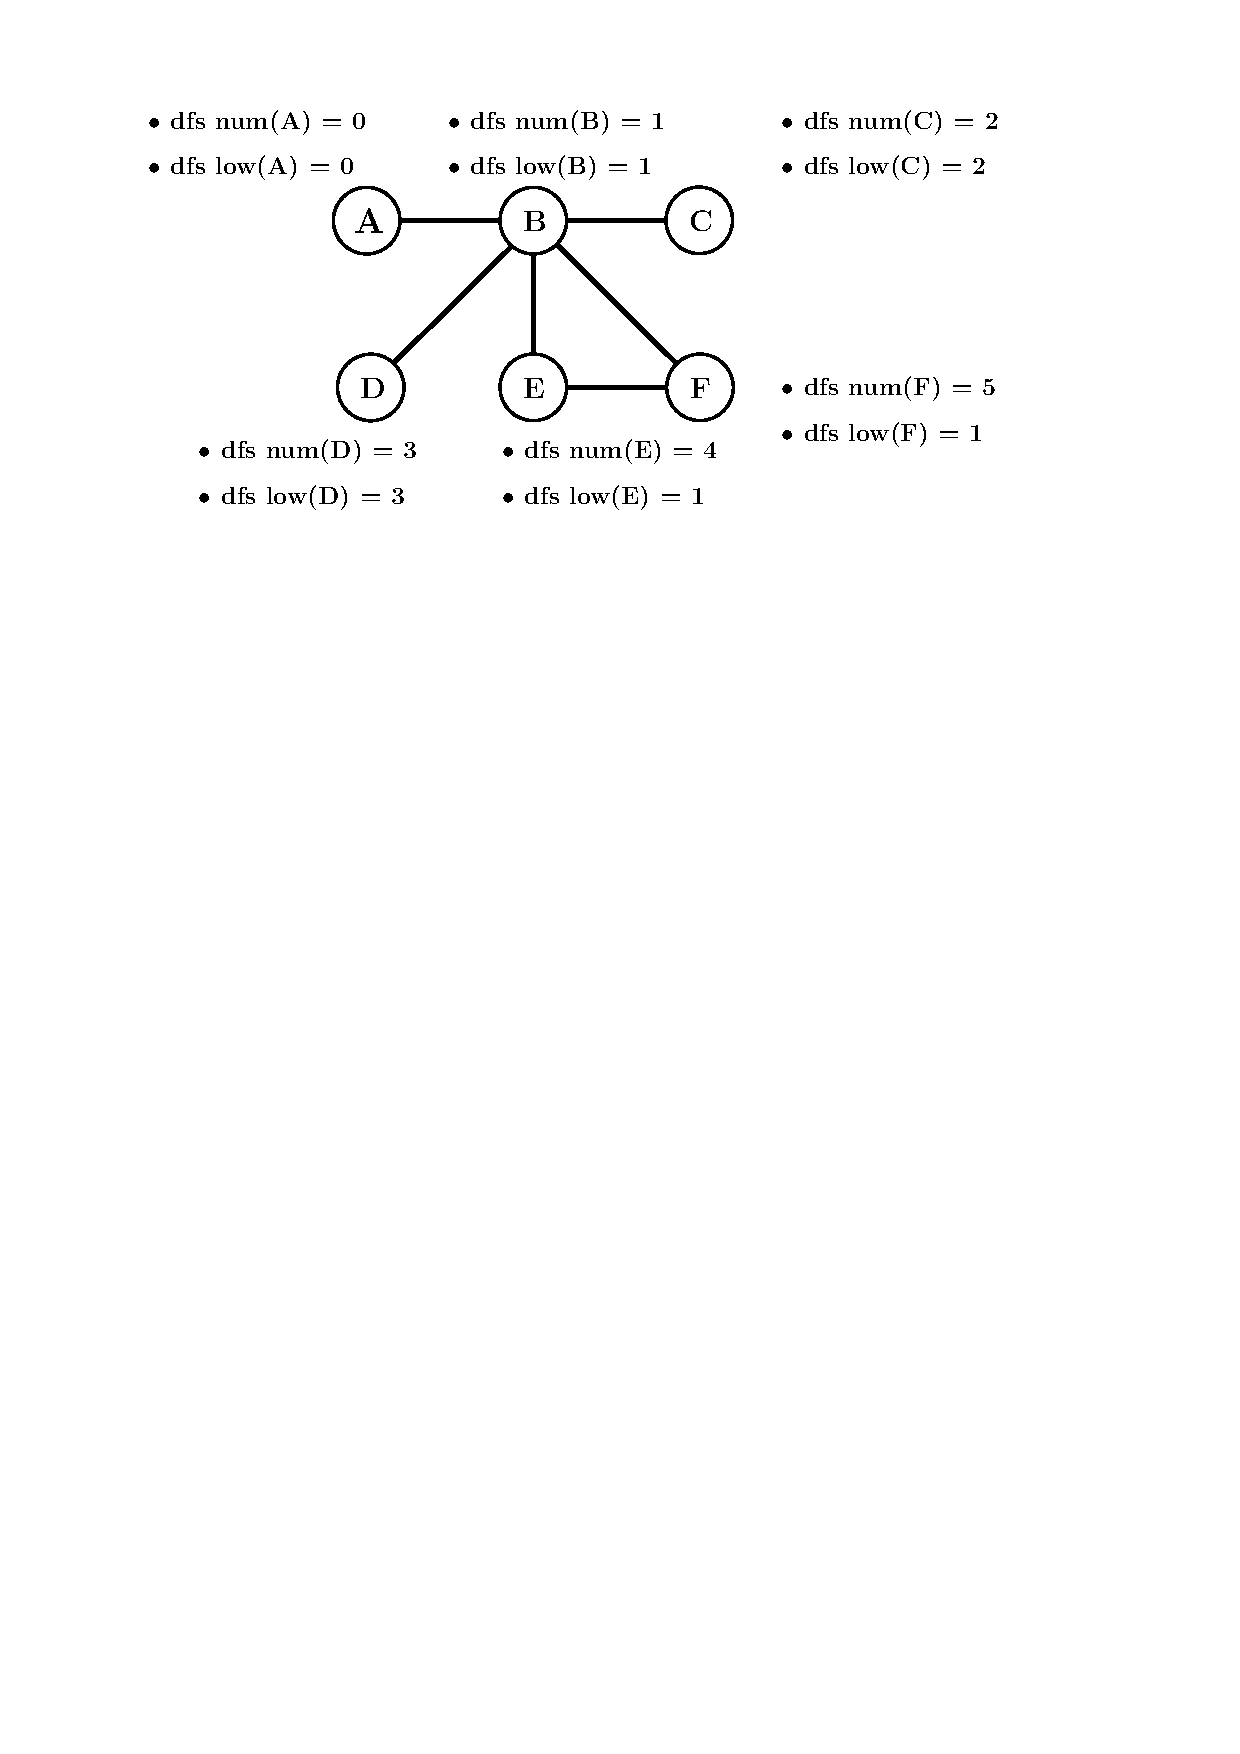
\includegraphics[scale = 0.75]{Bruecke_Separator_Algo.pdf}
\end{frame}